% This text is proprietary.
% It's a part of presentation made by myself.
% It may not used commercial.
% The noncommercial use such as private and study is free
% Nov. 2006
% Author: Sascha Frank 
% University Freiburg 
% www.informatik.uni-freiburg.de/~frank/
%
% additional usepackage{beamerthemeshadow} is used
%  
%  \beamersetuncovermixins{\opaqueness<1>{25}}{\opaqueness<2->{15}}
%  with this the elements which were coming soon were only hinted
\documentclass{beamer}
%\usepackage{beamerthemesplit}
\usepackage{asymptote}
\usepackage[update,prepend]{epstopdf}
\usepackage{subfigure}
%\usepackage{cite}
%\usepackage[cmex10]{amsmath}
\usepackage{amsfonts}
\usepackage{url}
\usepackage{pgf}
\usepackage{tikz}
\usetikzlibrary{arrows,chains,matrix,positioning,scopes}
%
\makeatletter
\tikzset{join/.code=\tikzset{after node path={%
\ifx\tikzchainprevious\pgfutil@empty\else(\tikzchainprevious)%
edge[every join]#1(\tikzchaincurrent)\fi}}}
\makeatother
%
\tikzset{>=stealth',every on chain/.append style={join},
         every join/.style={->}}
\tikzstyle{labeled}=[execute at begin node=$\scriptstyle,
   execute at end node=$]
\usepackage[style=ieee]{biblatex}
\addbibresource{presentation}
%\ExecuteBibliographyOptions{numeric-comp}

\def\docversion{Notes Version 0.1}

\usetheme{Luebeck}
\usecolortheme{lily}
\usefonttheme{serif}
\title{Image Processing}  
\author{Dr. Travis W. Axtell \\ \emph{travis.axtell@gmail.com}}
\institute{Mentor for FRC Team 612 --- Chantilly, VA \\ 
\quad\quad\quad\, FRC Team 
2035 --- 
Carmel, CA \\ \quad\quad\quad\quad\quad\quad FRC Team 5104 --- Pacific Grove, 
CA}
\date{\docversion\\ \today} 

\addtobeamertemplate{footnote}{}{\vspace{2ex}}

\setbeamercolor{block title}{use=structure,fg=white,bg=blue!75!black}
\setbeamercolor{block body}{use=structure,fg=black,bg=black!20!white}
\setbeamertemplate{blocks}[rounded][shadow=true]
%\setbeamertemplate{blocks}

\begin{document}

\frame{\titlepage} 

\frame{\frametitle{Table of contents}\tableofcontents} 


\section{Introduction} 
\frame{ 
\frametitle{How to read these notes}
\begin{itemize}
\item Underlined terms are concepts you should strive to understand, with the 
goal of being able to explain the concepts to others.
\item Investigate the meaning of new math notation.  Wikipedia can help --- see 
\url{https://en.wikipedia.org/wiki/List_of_mathematical_symbols}.
\item I am available for discussions when you need help.
\end{itemize}
}

\subsection{Formats}
\frame{ 
\frametitle{Modern file formats of interest}
Raster
\begin{itemize}
\item JPEG (JPG)
\item PNG
\item WEBP
\item GIF
\item RAW
\end{itemize}

Vector
\begin{itemize}
\item SVG
\item PDF
\end{itemize}

There are benefits to each format.  These notes discuss raster images.
}
%\begin{figure}
%	\includegraphics[scale=0.4]{SMT}
%	\caption{3-meter Segmented Mirror Telescope housed at Naval Postgraduate 
%School}
%\end{figure}
%}

\subsection{Definitions}
\frame{\frametitle{Raster Image Definitions}
\begin{columns}
\begin{column}{0.65\textwidth}
\begin{itemize}
\item A \underline{Scene}: $I(x,y)$ in continuous, physical coordinates $x$ and 
$y$.
\item An \underline{Image}: $I[n_1, n_2]$
of dimensions $N_1 \times N_2$ (width $\times$ height), where $n_1 \in \{1, 2, 
\dots, N_1 \}$
and $n_2\in \{1, \dots, N_2\}$ are all integers.
\begin{block}{Sampling}
$I[n_1, n_2] \equiv  I(n_1 \Delta x, n_2 \Delta y)$ \\
The image contains \underline{samples} of the scene using sampling intervals 
$\Delta x$ and $\Delta y$.
\end{block}
\item A \underline{Pixel} resides at every $[n_1, n_2]$ index.  
%This grid follows the left-handed coordinate system convention.
\end{itemize}
\end{column}
\begin{column}{0.35\textwidth}
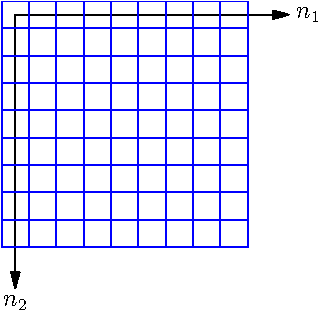
\includegraphics[width=0.9\textwidth]{coordinateframe}
\end{column}
\end{columns}
}

\frame{\frametitle{Image Processing Algorithm}
An image processing \underline{algorithm} uses the image as the input, performs 
computations, and outputs information.  Potential outputs include:
\begin{itemize}
\item Determine if an object is in the image [True/False]
\item Count objects in the image [\#]
\item Calculate the centroid of an object [$n_1, n_2$ coordinates]
\item Estimate $\Delta x$ and $\Delta y$ or physical quantities 
[\emph{e.g.} meters]
\end{itemize} 

\begin{figure}
\centering
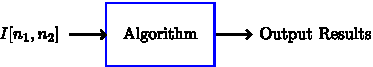
\includegraphics[keepaspectratio]{blockdiagram}
\end{figure}

This information can be used for other purposes, such as \underline{control} of 
a robot.
}

\subsection{Pixels}

\frame{\frametitle{Pixels}
Recall: $I[n_1, n_2]$ is an image that contains pixels.
\vspace{0.25cm}

How do we represent a pixel \underline{quantatively}?
}

\frame{ 
\frametitle{Pixels, round one}
%Recall: $I[n_1, n_2]$ is an image that contains pixels.
%\vspace{0.25cm}

If we make every pixel contain one number, then we can render a \underline{gray 
scale} or \underline{monochrome}\footnote{Assumes single-color light source.} 
image.

\begin{figure}
\centering
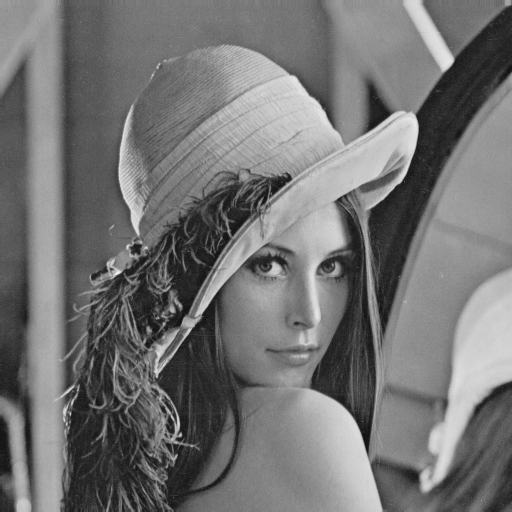
\includegraphics[scale=0.2]{LennaGray} \hspace{0.1cm}
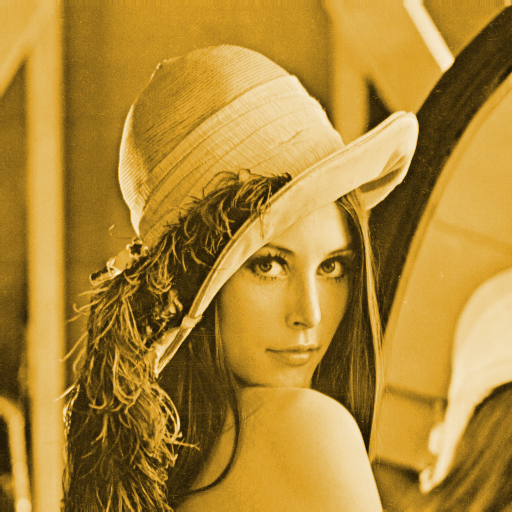
\includegraphics[scale=0.2]{LennaMono}
\caption{This image of Lena S\"{o}derberg is famous as a standard test from 
image processing literature.}
\end{figure}
}

\frame{ 
\frametitle{Pixels, round two}
%Recall: $I[n_1, n_2]$ is an image that contains pixels.
%\vspace{0.25cm}

If we make every pixel contain several numbers, then we can render a 
\underline{color} image.  Color images are stored in separate 
\underline{channels}, such as Red, Green, Blue (RGB). 

\begin{figure}
\centering
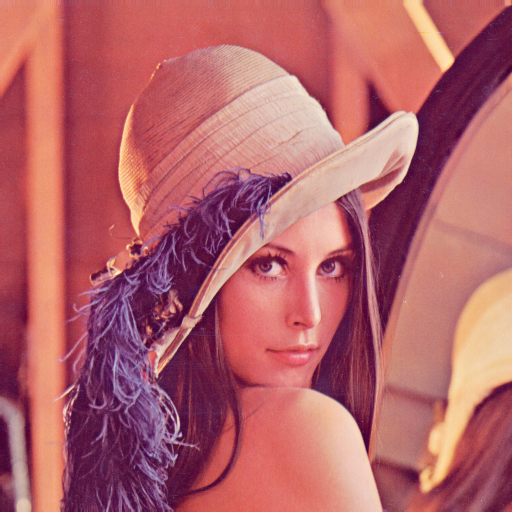
\includegraphics[scale=0.2]{Lenna}
\caption{The Lena image is composed of 3 channels.}
\end{figure}
}

\frame{ 
\frametitle{Pixels, round three}
%Recall: $I[n_1, n_2]$ is an image that contains pixels.
%\vspace{0.25cm}

Fact: Since \underline{digital} images $I[n_1, n_2]$ are stored on computers, 
pixels 
are efficiently represented as \underline{unsigned} integers. 

\vspace{0.25cm}
JPG images commonly use 8 bits per sample per channel --- represented as 
\underline{decimal} 0 to 255 
or \underline{hexadecimal} 0x00 to 0xFF.  Some advanced applications 
use 12, 14, or 24 bits, \emph{i.e.} medical imaging.

\vspace{0.25cm}
RAW images use as many bits as the hardware sensor, and this is why each 
manufacturer has unique RAW formats.

}

\frame{\frametitle{Pixels, review}
Recall: $I[n_1, n_2]$ is an image that contains pixels.
\vspace{0.25cm}

What \underline{information} is \underline{encoded} in pixels?

\begin{itemize}
\item Color
\item Spatial ($x$, $y$, and depth $z$)
\item Bit-depth
\item Camera location/field of view
\item Motion of the camera/objects
\item Sensor noise statistics
\item ...
\end{itemize} 
}

\section{Colors}
\frame{ 
\frametitle{Color in raster images}
Should we only use Red, Green, Blue?
\vspace{0.25cm}
\\
Paper Printers use Cyan, Magenta, Yellow, and Black (or Key) --- CMYK.
\vspace{0.25cm}
\\
Computer vision uses Hue, Saturation, Lightness or Value --- HSL and HSV.
\vspace{0.5cm}
\\
Why are there multiple \underline{color models}?
}

\section{RoboRealm software}

\frame{ 
\frametitle{RoboRealm}
\begin{itemize}
\item Can be installed by students for a 30-day evaluation for free in the 
off-season.
\item Important to practice algorithm development now before the season!
\end{itemize}

\centering
\url{http://www.roborealm.com/FRC2014/}

Click Trial Copy link on the page.
}

\frame{ 
\frametitle{RoboRealm start screen}
%\begin{figure}
\centering
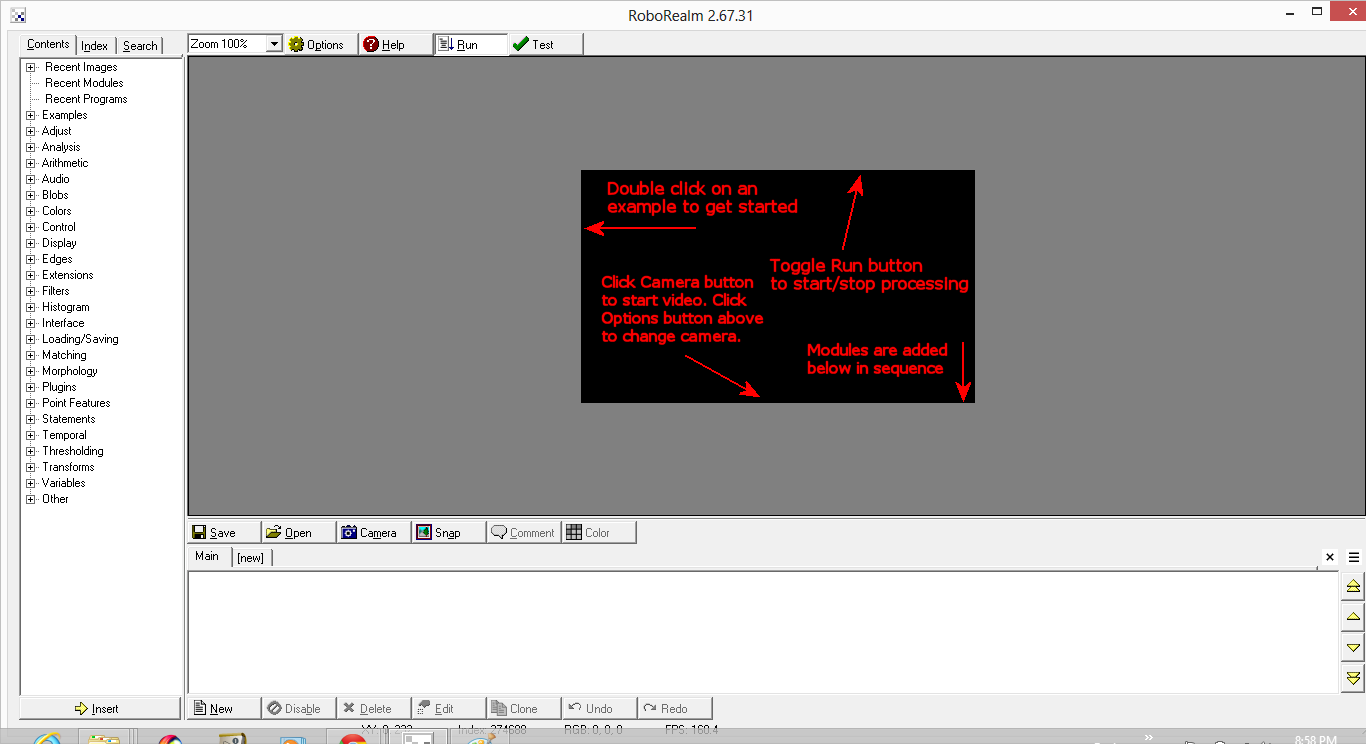
\includegraphics[width=\linewidth,height=\textheight,keepaspectratio]{RoboRealm1}
%\caption{The Lena image is composed of 3 channels.}
%\end{figure}
}

\frame{ 
\frametitle{RoboRealm with an example image}
%\begin{figure}
\centering
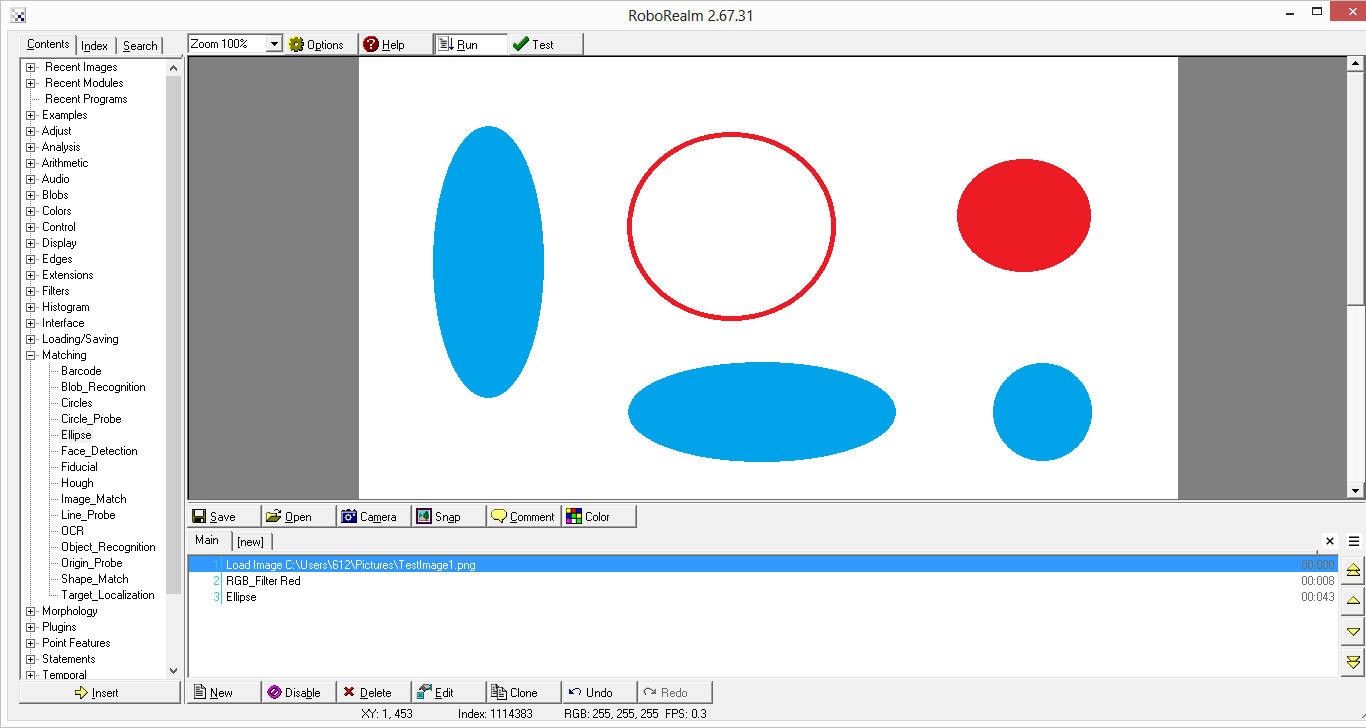
\includegraphics[width=\linewidth,height=\textheight,keepaspectratio]{RoboRealm2}
%\caption{The Lena image is composed of 3 channels.}
%\end{figure}
}

\frame{ 
\frametitle{RoboRealm sequence of steps}
The left column shows potential steps that can be applied.

\begin{enumerate}
\item First step is to load an image (look under Loading/Saving on the left 
list)
\item Next steps are to perform math steps on the image, potentially isolating 
a color region (by the \underline{Filters} or Colors items) or so 
forth.
\item Final steps will be to calculate information and provide to the robot, 
perhaps by NetworkTables or general network communication. 
\end{enumerate}

There's more than one sequence of steps to perform the same result.  Some 
approaches might be more \underline{robust} (or brittle!) than others.
}

\section{Vision resources}
\frame{ 
\frametitle{Vision resources}
[1] \href{http://www.chiefdelphi.com/media/papers/2854}{\underline{Vision 
Processing and Frisbee Shooter Controller Design}}

[2] \href{http://programmingcomputervision.com/}{\underline{Programming 
Computer Vision with Python}}

\vspace{0.5cm}
The first paper shows steps performed in NI Vision Assistant, but the same 
steps can be found in RoboRealm.  The second reference has sections that should 
be interesting to read.

}

\end{document}
